% Дополнительные задачи темы 3.2.2, приведённые к оформлению курса.
% Компилировать XeLaTeX.
\documentclass[12pt,a4paper]{article}
\usepackage{egephys-style}
\usepackage{microtype}
\usepackage[european]{circuitikz}
\ctikzset{resistors/scale=0.8, bipoles/length=1.1cm}
\emergencystretch=3em

\tikzset{
  Fvec/.style={-{Stealth[scale=0.9]},brandSecondary,very thick},
  vvec/.style={-{Stealth[scale=0.9]},brandAccent,very thick},
}

\begin{document}

\begin{taskmedium}
\textbf{1.} Катушка №~1 включена в электрическую цепь, состоящую из источника постоянного напряжения
и реостата. Катушка №~2 помещена внутрь катушки №~1, и её обмотка замкнута. Вид электрической цепи с
торца катушек схематично представлен на рисунке.

Из приведённого ниже списка выберите все верные утверждения, характеризующие процессы, которые
происходят в цепи и катушках при перемещении ползунка реостата влево. ЭДС самоиндукции пренебречь.

\nopagebreak\smallskip
\begin{center}
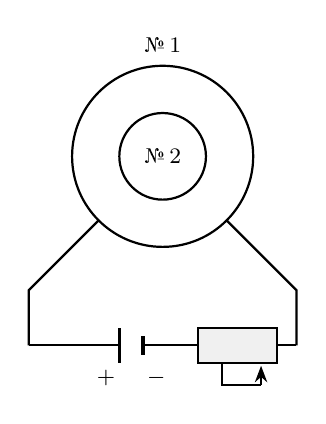
\begin{tikzpicture}[scale=1.0, font=\small, >=Stealth]
  % катушка 1 (внешняя) и катушка 2 (внутренняя) — вид с торца
  \draw[thick] (0,0) circle (1.15);
  \draw[thick] (0,0) circle (0.55);
  \node[font=\footnotesize] at (0,1.42) {№\,1};
  \node[font=\footnotesize] at (0,0)    {№\,2};
  % выводы внешней катушки в цепь
  \draw[thick] (-0.81,-0.81) -- (-1.7,-1.7) -- (-1.7,-2.4);
  \draw[thick] (0.81,-0.81)  -- (1.7,-1.7)  -- (1.7,-2.4);
  % источник и реостат
  \draw[thick] (-1.7,-2.4) -- (-0.55,-2.4);
  \draw[very thick] (-0.55,-2.62) -- (-0.55,-2.18);
  \draw[very thick] (-0.25,-2.52) -- (-0.25,-2.28);
  \node[font=\footnotesize] at (-0.72,-2.82) {$+$};
  \node[font=\footnotesize] at (-0.08,-2.82) {$-$};
  \draw[thick] (-0.25,-2.4) -- (0.45,-2.4);
  \draw[thick,fill=gray!12] (0.45,-2.62) rectangle (1.45,-2.18);
  \draw[thick] (0.75,-2.62) -- (0.75,-2.90) -- (1.25,-2.90);
  \draw[thick,-{Stealth[scale=0.9]}] (1.25,-2.90) -- (1.25,-2.66);
  \draw[thick] (1.45,-2.4) -- (1.7,-2.4);
\end{tikzpicture}
\end{center}

1) Модуль вектора индукции магнитного поля, созданного катушкой №~1, увеличивается.\\
2) В катушке №~2 индукционный ток направлен по часовой стрелке.\\
3) Сила тока в катушке №~1 уменьшается.\\
4) Вектор индукции магнитного поля, созданного катушкой №~2 в её центре, направлен от наблюдателя.\\
5) Модуль магнитного потока, созданного катушкой №~1 и пронизывающего катушку №~2, увеличивается.
\kim{14}
\end{taskmedium}

\begin{taskadvanced}
\textbf{2.} По двум горизонтально расположенным параллельным проводящим рельсам с пренебрежимо малым
сопротивлением, замкнутым на конденсатор, поступательно и равномерно со скоростью $v=1$~м/с скользит
проводящий стержень. Расстояние между рельсами $l=80$~см. Рельсы со стержнем находятся в вертикальном
однородном магнитном поле с индукцией $B=5$~Тл (см. рисунок, вид сверху). Энергия электрического поля
конденсатора через достаточно большой промежуток времени от начала движения $W=40$~мкДж. Какова
электроёмкость конденсатора $C$? Рельсы закреплены на диэлектрической подложке.

\nopagebreak\smallskip
\begin{center}
\begin{tikzpicture}[scale=1.0, font=\small, >=Stealth]
  % поле «от нас»
  \foreach \x in {0,1,2,3,4}\foreach \y in {0,1}{
    \draw[brandPrimary,thin] ({0.6+\x*0.85},{0.35+\y*0.85}) circle (0.09);
    \draw[brandPrimary,thin] ({0.6+\x*0.85-0.063},{0.35+\y*0.85-0.063})
                          -- ({0.6+\x*0.85+0.063},{0.35+\y*0.85+0.063});
    \draw[brandPrimary,thin] ({0.6+\x*0.85-0.063},{0.35+\y*0.85+0.063})
                          -- ({0.6+\x*0.85+0.063},{0.35+\y*0.85-0.063});}
  \node[brandPrimary,font=\footnotesize] at (4.6,-0.35) {$\vec B$};
  % рельсы
  \draw[thick] (0,0) -- (4.9,0);
  \draw[thick] (0,1.55) -- (4.9,1.55);
  % конденсатор слева
  \draw[thick] (0,0) -- (0,0.60);
  \draw[thick] (0,1.55) -- (0,0.95);
  \draw[very thick] (-0.30,0.60) -- (0.30,0.60);
  \draw[very thick] (-0.30,0.95) -- (0.30,0.95);
  \node[font=\footnotesize] at (-0.55,0.78) {$C$};
  % стержень
  \draw[line width=2.6pt,brandAccent] (2.75,0) -- (2.75,1.55);
  \draw[vvec] (2.95,0.78) -- (3.85,0.78) node[right,font=\footnotesize,black] {$\vec v$};
  \draw[<->,gray] (2.45,0) -- (2.45,1.55) node[midway,fill=white,font=\footnotesize,black] {$l$};
\end{tikzpicture}
\end{center}
\kim{23}
\end{taskadvanced}

\begin{taskadvanced}
\textbf{3.} Металлический стержень, согнутый в виде буквы П, закреплён в горизонтальном положении
(см. рисунок). На параллельные стороны стержня опирается концами перпендикулярная перемычка
прямоугольного поперечного сечения массой $300$~г и длиной $1$~м. Вся система находится в однородном
вертикальном магнитном поле с индукцией $0{,}2$~Тл. Под действием постоянной горизонтальной силы
$F=1{,}6$~Н перемычка движется с постоянной скоростью $1{,}5$~м/с. Определите сопротивление
перемычки. Коэффициент трения между стержнем и перемычкой равен $0{,}2$. Сопротивлением стержня
пренебречь. Сделайте рисунок с указанием сил, действующих на перемычку.

\nopagebreak\smallskip
\begin{center}
\begin{tikzpicture}[scale=1.0, font=\small, >=Stealth]
  % поле «от нас» (вертикальное, вид сверху)
  \foreach \x in {0,1,2,3,4}\foreach \y in {0,1}{
    \draw[brandPrimary,thin] ({0.55+\x*0.85},{0.35+\y*0.85}) circle (0.09);
    \draw[brandPrimary,thin] ({0.55+\x*0.85-0.063},{0.35+\y*0.85-0.063})
                          -- ({0.55+\x*0.85+0.063},{0.35+\y*0.85+0.063});
    \draw[brandPrimary,thin] ({0.55+\x*0.85-0.063},{0.35+\y*0.85+0.063})
                          -- ({0.55+\x*0.85+0.063},{0.35+\y*0.85-0.063});}
  \node[brandPrimary,font=\footnotesize] at (4.55,-0.35) {$\vec B$};
  % П-образный стержень
  \draw[line width=1.8pt] (0,0) -- (4.8,0);
  \draw[line width=1.8pt] (0,1.55) -- (4.8,1.55);
  \draw[line width=1.8pt] (0,0) -- (0,1.55);
  % перемычка
  \draw[line width=2.8pt,brandAccent] (2.60,0) -- (2.60,1.55);
  \draw[Fvec] (2.80,0.78) -- (3.80,0.78) node[right,font=\footnotesize,black] {$\vec F$};
  \draw[<->,gray] (2.30,0) -- (2.30,1.55) node[midway,fill=white,font=\footnotesize,black] {$l$};
\end{tikzpicture}
\end{center}
\kim{25}
\end{taskadvanced}

\begin{taskadvanced}
\textbf{4.} Металлический стержень, согнутый в виде буквы П, закреплён в горизонтальном положении
(см. рисунок к задаче~3). На параллельные стороны стержня опирается концами перпендикулярная
перемычка прямоугольного поперечного сечения массой $370$~г и длиной $1$~м. Сопротивление перемычки
равно $0{,}025$~Ом. Вся система находится в однородном вертикальном магнитном поле с индукцией
$0{,}1$~Тл. Какую горизонтальную силу нужно приложить к перемычке, чтобы двигать её с постоянной
скоростью $2$~м/с, если коэффициент трения между стержнем и перемычкой равен $0{,}2$? Сопротивлением
стержня пренебречь. Сделайте рисунок с указанием сил, действующих на перемычку.
\kim{25}
\end{taskadvanced}

\begin{taskadvanced}
\textbf{5.} Квадратная рамка из медного провода с площадью поперечного сечения
$S_0=0{,}1$~мм$^2$ помещена в однородное поле электромагнита. На рисунке приведён график зависимости
от времени $t$ для проекции $B_n$ вектора индукции этого поля на перпендикуляр к плоскости рамки.
Какое количество теплоты выделяется в рамке за время $\tau=4$~с? Длина стороны рамки $l=10$~см.
Удельное сопротивление меди $\rho=1{,}7\cdot10^{-8}$~Ом$\cdot$м.

\nopagebreak\smallskip
\begin{center}
\begin{tikzpicture}[x=0.95cm, y=3.1cm, font=\small, >=Stealth]
  \foreach \t in {1,2,3,4,5}{\draw[gray!35,thin] (\t,-0.25) -- (\t,0.35);}
  \foreach \b in {-0.2,-0.1,0.1,0.2,0.3}{\draw[gray!35,thin] (0,\b) -- (5.6,\b);}
  \draw[-{Stealth[scale=0.8]},thick] (0,0) -- (6.2,0) node[below right] {$t$, с};
  \draw[-{Stealth[scale=0.8]},thick] (0,-0.28) -- (0,0.40) node[above] {$B_n$, Тл};
  \draw[ultra thick,brandPrimary] (0,0.3) -- (5,-0.2);
  \foreach \t in {1,2,4,5}{\node[below,font=\footnotesize] at (\t,0) {\t};}
  \foreach \b/\lab in {0.3/{0,3},0.2/{0,2},0.1/{0,1},-0.1/{-0,1},-0.2/{-0,2}}{
    \node[left,font=\footnotesize] at (0,\b) {\lab};}
  \node[below left,font=\footnotesize] at (0,0) {0};
\end{tikzpicture}
\end{center}
\kim{25}
\end{taskadvanced}

\newpage
\hwlevel{Ответы}{brandSecondary}

\textbf{1.} \rule{4cm}{0.4pt}\\[0.3em]
\textbf{2.} $C=5$~мкФ\\[0.3em]
\textbf{3.} $R=0{,}06$~Ом\\[0.3em]
\textbf{4.} $F=1{,}54$~Н\\[0.3em]
\textbf{5.} $Q\approx59$~мкДж

\medskip
\textbf{Эталоны Части 2.}

\begin{solutionbox}
\textbf{Задание 23 (задача 2).}

\textbf{Решение.} При движении стержня в магнитном поле возникает ЭДС индукции
\[ \mathcal{E}=Bvl=5\cdot1\cdot0{,}8=4\ \text{В}. \]
Через большой промежуток времени конденсатор полностью зарядится, ток в цепи прекратится, и падения
напряжения на сопротивлениях не будет. Значит напряжение на конденсаторе равно ЭДС: $U=\mathcal{E}=4$~В.

Из энергии электрического поля конденсатора
\[ W=\frac{CU^{2}}{2}\quad\Longrightarrow\quad
C=\frac{2W}{U^{2}}=\frac{2\cdot40\cdot10^{-6}}{16}=5\cdot10^{-6}\ \text{Ф}. \]
\answer{$C=5$~мкФ}
\end{solutionbox}

\begin{solutionbox}
\textbf{Задание 25 (задача 3).}

\textbf{Решение.} Перемычка движется равномерно, значит равнодействующая всех сил равна нулю. Вдоль
направления движения на неё действуют: приложенная сила $\vec F$, сила трения $\vec F_{\text{тр}}$ и
сила Ампера $\vec F_A$, обе направленные против движения:
\[ F=F_{\text{тр}}+F_A . \]
Сила трения $F_{\text{тр}}=\mu mg=0{,}2\cdot0{,}3\cdot10=0{,}6$~Н.

При движении возникает ЭДС $\mathcal{E}=Bvl$, ток $I=\dfrac{Bvl}{R}$ и сила Ампера
\[ F_A=BIl=\frac{B^{2}l^{2}v}{R}. \]
Отсюда
\[ R=\frac{B^{2}l^{2}v}{F-F_{\text{тр}}}
=\frac{0{,}2^{2}\cdot1^{2}\cdot1{,}5}{1{,}6-0{,}6}=\frac{0{,}06}{1}=0{,}06\ \text{Ом}. \]
\answer{$R=0{,}06$~Ом}
\end{solutionbox}

\begin{critbox}
\textbf{3 балла} — приведено полное верное решение: сделан рисунок с силами, записано условие
равномерного движения, выражена сила Ампера через ЭДС индукции, найдено сопротивление.\\[0.3em]
\textbf{2 балла} — ход решения верен, но допущена ошибка в вычислениях либо не сделан
рисунок.\\[0.3em]
\textbf{1 балл} — записаны условие равновесия и формула силы Ампера, но решение не доведено до
ответа.\\[0.3em]
\textbf{0 баллов} — все случаи решения, не соответствующие критериям выше.
\end{critbox}

\begin{solutionbox}
\textbf{Задание 25 (задача 4).}

\textbf{Решение.} Как и в предыдущей задаче, при равномерном движении
$F=F_{\text{тр}}+F_A$, где
\[ F_{\text{тр}}=\mu mg=0{,}2\cdot0{,}37\cdot10=0{,}74\ \text{Н},\qquad
F_A=\frac{B^{2}l^{2}v}{R}=\frac{0{,}1^{2}\cdot1^{2}\cdot2}{0{,}025}=0{,}8\ \text{Н}. \]
Тогда
\[ F=0{,}74+0{,}8=1{,}54\ \text{Н}. \]
\answer{$F=1{,}54$~Н}
\end{solutionbox}

\begin{solutionbox}
\textbf{Задание 25 (задача 5).}

\textbf{Решение.} По графику индукция убывает равномерно от $0{,}3$~Тл при $t=0$ до $-0{,}2$~Тл при
$t=5$~с, поэтому скорость её изменения постоянна:
\[ \left|\frac{\Delta B}{\Delta t}\right|=\frac{0{,}3-(-0{,}2)}{5}=0{,}1\ \text{Тл/с}. \]
Площадь рамки $S=l^{2}=0{,}01$~м$^2$ не меняется, значит модуль ЭДС индукции
\[ \mathcal{E}=S\left|\frac{\Delta B}{\Delta t}\right|=0{,}01\cdot0{,}1=10^{-3}\ \text{В}. \]
Сопротивление рамки — это сопротивление провода длиной в четыре стороны:
\[ R=\frac{\rho\cdot4l}{S_0}=\frac{1{,}7\cdot10^{-8}\cdot0{,}4}{0{,}1\cdot10^{-6}}=0{,}068\ \text{Ом}. \]
Количество теплоты за время $\tau$:
\[ Q=\frac{\mathcal{E}^{2}}{R}\,\tau=\frac{10^{-6}}{0{,}068}\cdot4\approx5{,}9\cdot10^{-5}\ \text{Дж}. \]
\answer{$Q\approx59$~мкДж}
\end{solutionbox}

\begin{critbox}
\textbf{3 балла} — приведено полное верное решение: по графику найдена скорость изменения индукции,
вычислена ЭДС через площадь рамки, найдено сопротивление рамки по длине всех четырёх сторон, получен
верный числовой ответ.\\[0.3em]
\textbf{2 балла} — ход решения верен, но допущена ошибка в вычислениях либо в длине провода (взята
одна сторона вместо четырёх).\\[0.3em]
\textbf{1 балл} — записаны формулы ЭДС индукции и закона Джоуля — Ленца, но решение не доведено до
ответа.\\[0.3em]
\textbf{0 баллов} — все случаи решения, не соответствующие критериям выше.
\end{critbox}

\end{document}